\section{Results}

\begin{figure}
  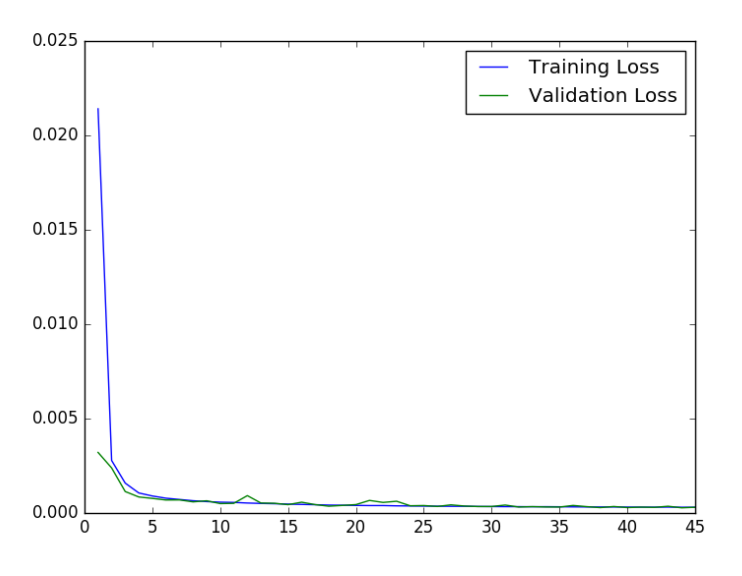
\includegraphics[width=\linewidth]{images/validationloss.png}
  \caption{Training and Validation loss of depth map}
  \label{fig:boat1}
\end{figure}

The neural network was able to accurately estimate the depth parity given 2 input stereo images. The validation loss was calculated by comparing the ground truth depth map generated using Blender against the predicted depth map obtained from the Neural Network.

Validation loss was determined to be in the order of 10-3 . 

\begin{figure}
  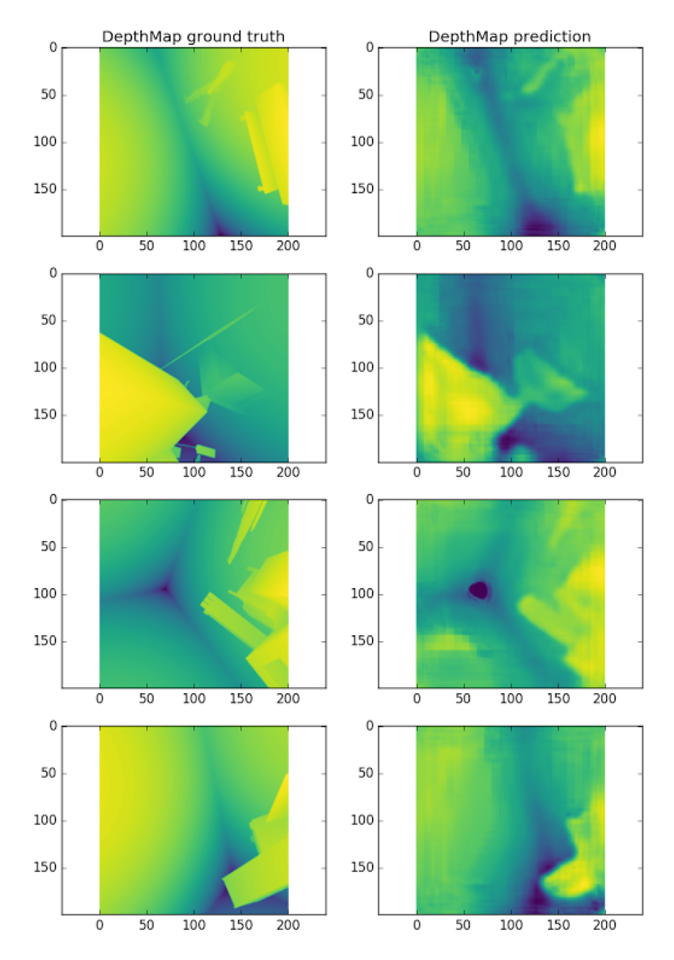
\includegraphics[width=\linewidth]{images/depthmap2.png}
  \caption{Performance of depth map on simulated images}
  \label{fig:depthmap2}
\end{figure}

The performance of the algorithm with different heuristics is given in Table 1.
 
\begin{table}[h!]
  \centering
  \caption{Performance Metrics}
  \label{tab:table1}
  \begin{threeparttable}
  \begin{tabular}{cccccc}
    \toprule
        \textbf{S No}. & \textbf{Human Baseline} & {\boldm $\mathrm{M}_{\mathrm{Man}}$} & {\boldm $\mathrm{M}_{\mathrm{Euc}}$}  & {\boldm $\mathrm{R}_{\mathrm{Man}}$} & {\boldm $\mathrm{R}_{\mathrm{Euc}}$}\\
    \midrule
    	1 & 179 & 330 & 241 & 1.84 & 1.35\\
    	2 & 209 & 472 & 472 & 2.26 & 2.26\\
    	3 & 276 & 556 & 520 & 2.01 & 1.88\\
    	4 & 269 & 252 & 551 & 0.93 & 2.05\\
    	5 & 167 & 401 & 401 & 2.40 & 2.40\\
    	6 & 197 & 462 & 361 & 2.35 & 1.83\\
    	7 & 123 & 114 & 114 & 0.93 & 0.93\\
      \textbf{Median} &-&-&-& \textbf{ 2.01} & \textbf{1.88}\\
      \textbf{Average} &-&-&-& \textbf{1.81} & \textbf{1.80}\\
    \bottomrule
  \end{tabular}
  \begin{tablenotes}
    \item {\boldm $ \mathrm{S No.} $ }: Scenario number, with each scenario having different source and destination points.
    \item {\boldm $ \mathrm{Human}\:\mathrm{Baseline} $}: Step count of a human performing the experiment
    \item {\boldm $ \mathrm{M}_\mathrm{Man} $}: Step count of the control policy using Manhattan distance as heuristic.
    \item {\boldm $ \mathrm{M}_\mathrm{Euc} $}: Step count of the control policy using Euclidean distance as heuristic.
    \item {\boldm $ \mathrm{R}_\mathrm{Man} $}: Ratio of Manhattan to Baseline performance (Lower is Better)
    \item {\boldm $ \mathrm{R}_\mathrm{Euc} $}: Ratio of Euclidean to Baseline performance (Lower is Better)
  \end{tablenotes}
  \end{threeparttable}
\end{table}

The average relative performance of the Manhattan based heuristic was found to be 1.81

The median relative performance of the Manhattan based heuristic was found to be 2.01

The average relative performance of the Euclidean based heuristic was found to be 1.80

The median relative performance of the Euclidean based heuristic was found to be 1.88
 
The average metric is susceptible to outliers in observations and is hence a less reliable metric for evaluation. The median metric is able to circumvent this problem, and is thus a better measure of the relative performances of the heuristics in this situation.
  
The Euclidean heuristic equaled or outperformed the Manhattan heuristic on 85.71\% of the experiments, and is hence a better heuristic for evaluation.


\begin{figure}
  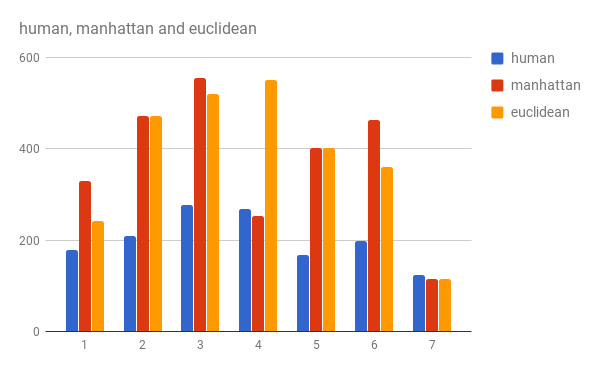
\includegraphics[width=\linewidth]{images/chart.png}
  \caption{Performance of heuristics vs humans}
  \label{fig:chart1}
\end{figure}